\documentclass[pdflatex,sn-mathphys]{sn-jnl}
\jyear{\year}

\usepackage{lipsum}

\raggedbottom

\begin{document}

\title[Modelagem de processo industrial de manufatura]{Modelagem de processo industrial de manufatura}

%\author*[1,2]{\pfx{Dr} \fnm{Joergen W.} \spfx{van der} \sur{Ploeg} \sfx{IV} \tanm{Poet Laureate} \dgr{MSc, PhD}}\email{iauthor@gmail.com}

\author[1]{\fnm{First} \sur{Author}}\email{iauthor@gmail.com}

\author[1]{\fnm{ii} \sur{Author}}\email{iiauthor@gmail.com}

\author[1]{\fnm{iii} \sur{Author}}\email{iiiauthor@gmail.com}

\affil[1]{\orgdiv{Programa de Pós-Graduação em Engenharia Elétrica}, \orgname{Universidade Tecnológica Federal do Paraná}, \orgaddress{\street{Via do Conhecimento}, \city{Pato Branco}, \postcode{85503-390}, \state{PR}, \country{Brasil}}}

\abstract{\lipsum[1-2]}

\keywords{SED, Industry 4.0, TCS}

\maketitle

\section{Introdução}

\subsection{Processo industrial de manufatura}
A Fig. \ref{fig:processo} apresenta uma visão da planta industrial a ser modelada e simulada.
A composição da planta é a seguinte:
\begin{itemize}
    \item Mesa centralizadora com teste de chapa;
    \item 5 robôs manipuladores;
    \item 4 prensas;
    \item Esteira para destinação final das peças;
\end{itemize}

TODO: descrever processo de manufatura

\begin{figure}[H]%
    \centering
    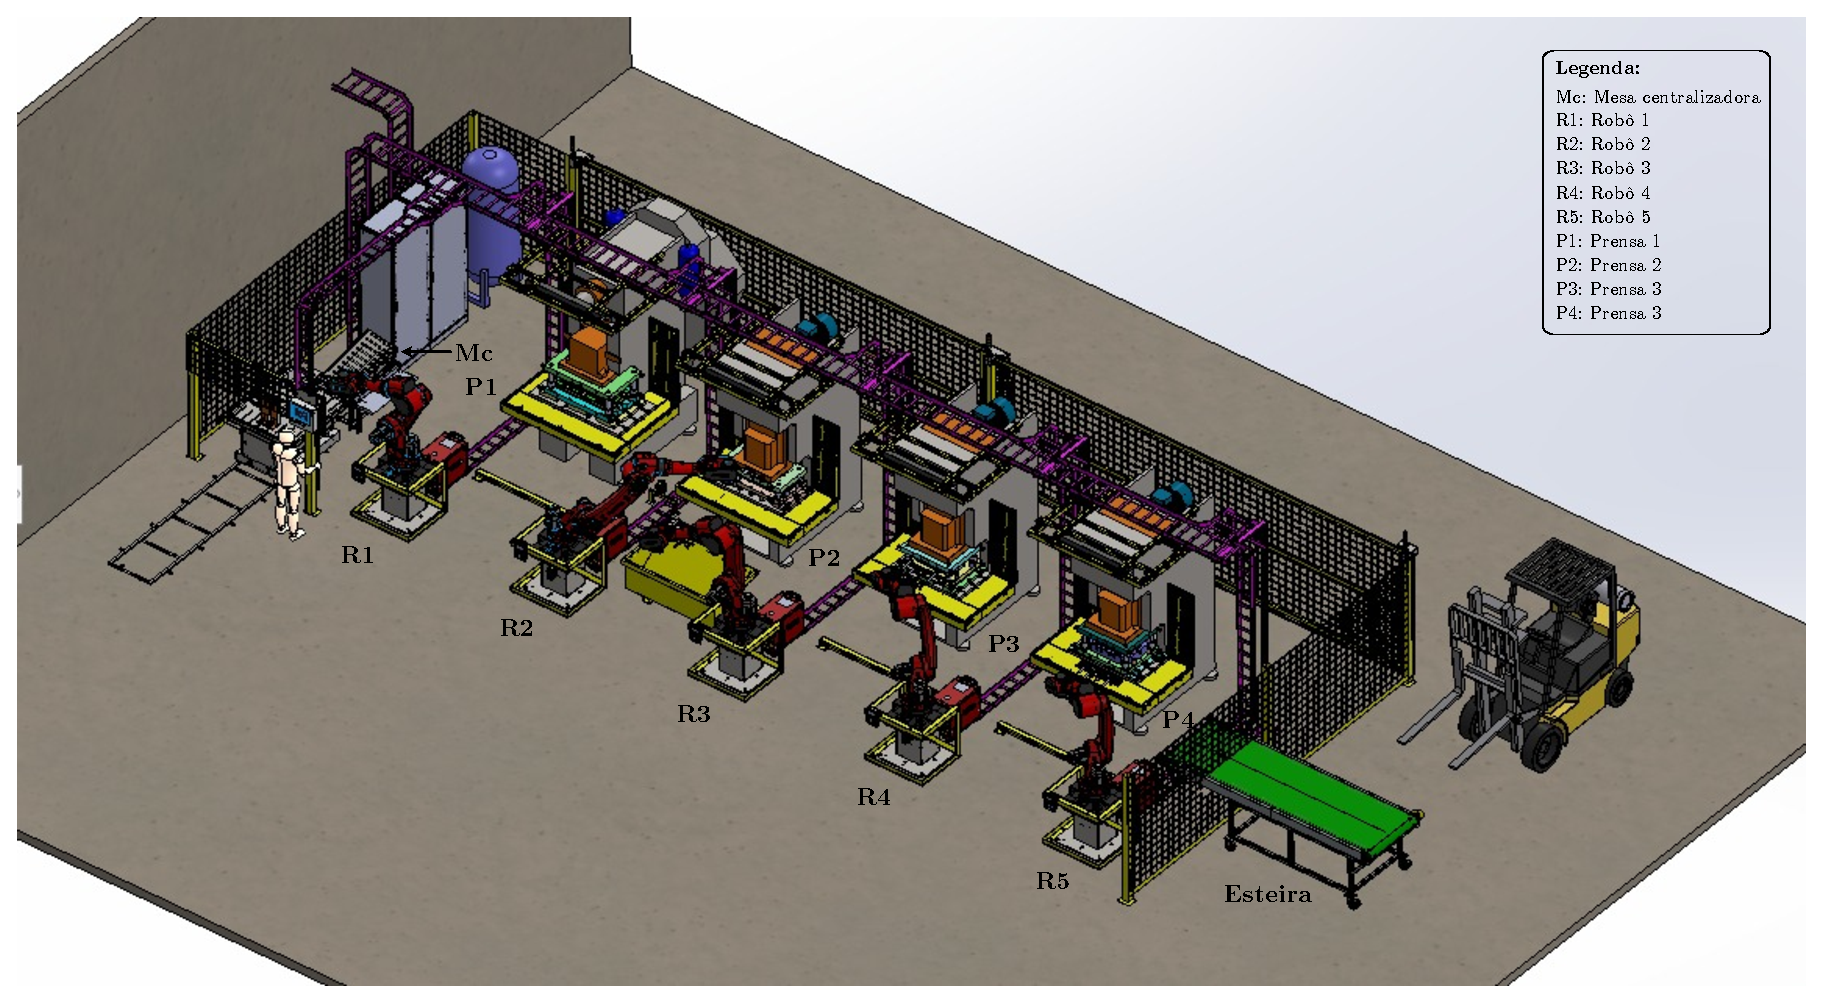
\includegraphics[width=0.8\textwidth]{imagens/processo.eps}
    \caption{Planta industrial}\label{fig:processo}
\end{figure}
%\input{capitulos/revisao_bibliografica.tex}
\section{Plantas}
Robo 1
\lipsum[1]
\begin{figure}[H]%
    \centering
    \includegraphics[width=0.9\textwidth]{imagens/robo_1.eps}
    \caption{Planta Robo 1}\label{fig:robo1}
\end{figure}

Robo 2
\lipsum[2]
\begin{figure}[H]%
    \centering
    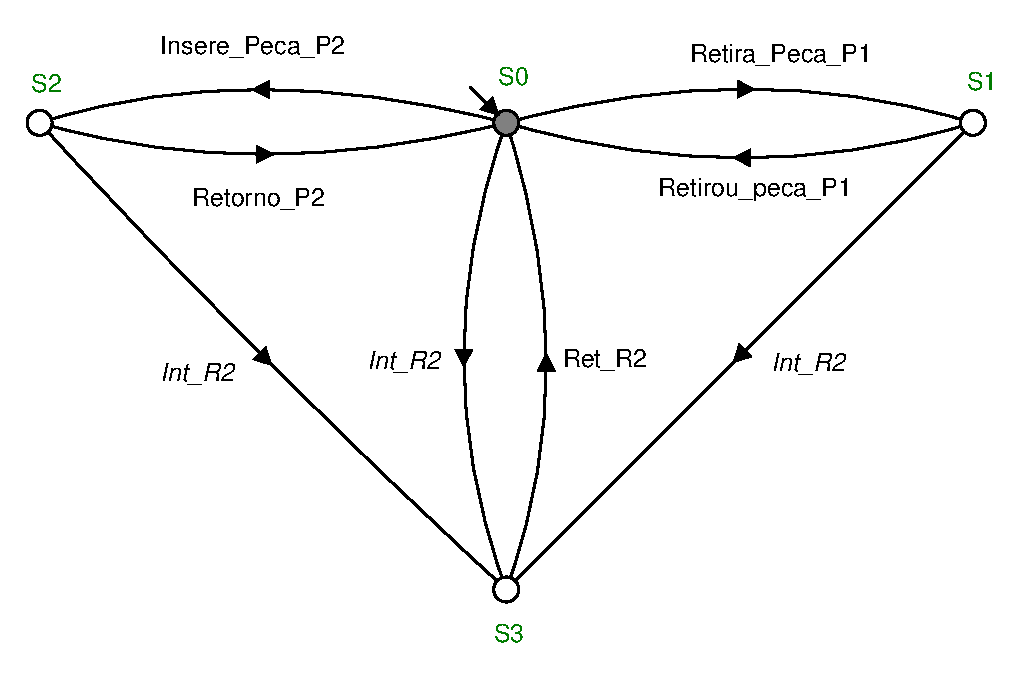
\includegraphics[width=0.9\textwidth]{imagens/robo_2.eps}
    \caption{Planta Robo 2}\label{fig:robo2}
\end{figure}

Robo 3
\lipsum[3]
\begin{figure}[H]%
    \centering
    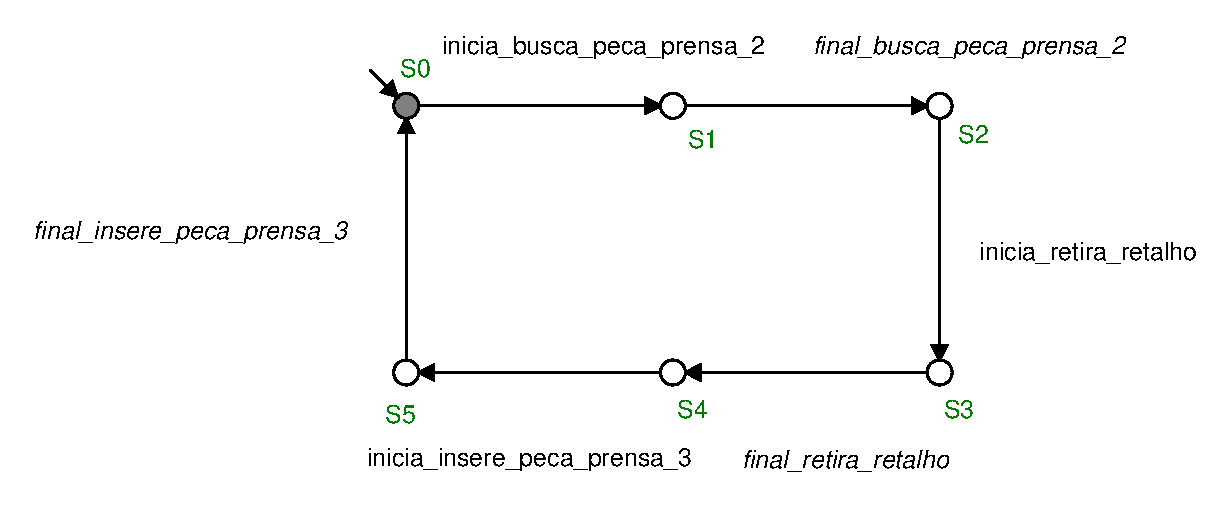
\includegraphics[width=0.9\textwidth]{imagens/robo_3.eps}
    \caption{Planta Robo 3}\label{fig:robo3}
\end{figure}

Robo 4
\lipsum[4]
\begin{figure}[H]%
    \centering
    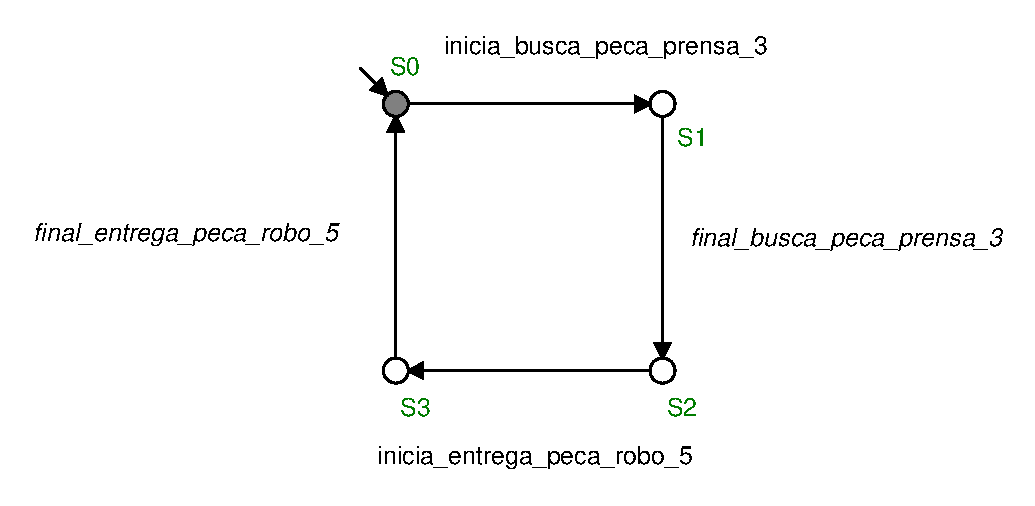
\includegraphics[width=0.9\textwidth]{imagens/robo_4.eps}
    \caption{Planta Robo 4}\label{fig:robo4}
\end{figure}

Robo 5
\lipsum[5]
\begin{figure}[H]%
    \centering
    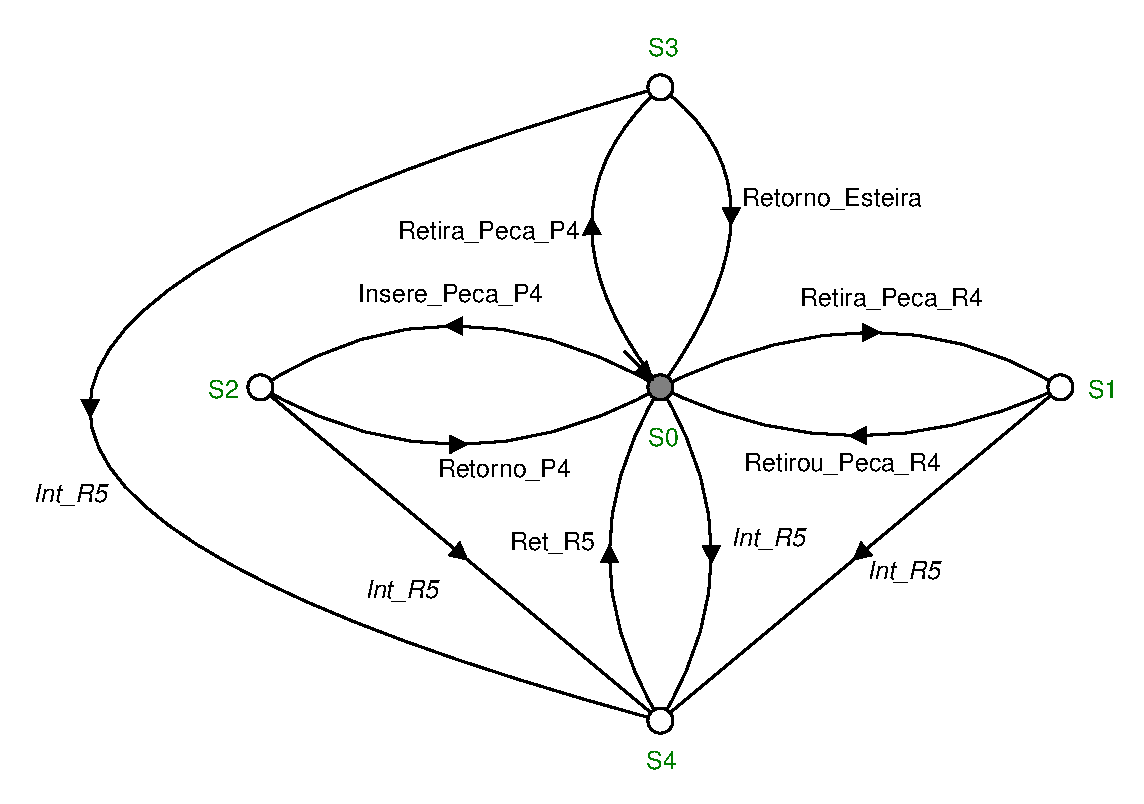
\includegraphics[width=0.9\textwidth]{imagens/robo_5.eps}
    \caption{Planta Robo 5}\label{fig:robo5}
\end{figure}

\lipsum[6]

Citação \cite{bib1} 123 456

\lipsum[7]

\section{Especificações}
\lipsum[1]
\begin{figure}[H]%
    \centering
    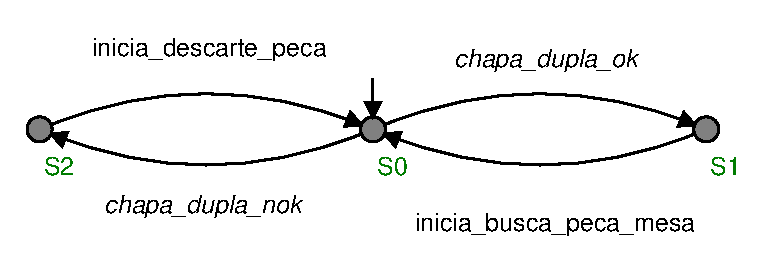
\includegraphics[width=0.9\textwidth]{imagens/E1_robo_1_chapa_dupla.eps}
    \caption{Planta Robo 5}\label{fig:robo5}
\end{figure}

\section{Conclusões}
TODO: explicar explosão do número de estados do modelo.

\bibliography{sn-bibliography}

\end{document}
